\documentclass{beamer}
\setbeamercovered{transparent}
\usepackage{appendixnumberbeamer}
%
% Choose how your presentation looks.
%
% For more themes, color themes and font themes, see:
% http://deic.uab.es/~iblanes/beamer_gallery/index_by_theme.html
%
\mode<presentation>
{
  \usetheme{Madrid}      % or try Darmstadt, Madrid, Warsaw, ...
  \usecolortheme{dolphin} % or try albatross, beaver, crane, ...
%   \usecolortheme{beaver} % or try albatross, beaver, crane, ...
  \usefonttheme{default}  % or try serif, structurebold, ...
  \setbeamertemplate{navigation symbols}{}
  \setbeamertemplate{caption}[numbered]
  \setbeamercolor{alerted text}{fg=red}
} 

\newcounter{saveenumi}
\newcommand{\seti}{\setcounter{saveenumi}{\value{enumi}}}
\newcommand{\conti}{\setcounter{enumi}{\value{saveenumi}}}

\resetcounteronoverlays{saveenumi}

\usepackage[czech]{babel}
\usepackage[utf8]{inputenc}

\title[Diplomová práca]{Lexikální analyzátor dialektu dotazovacího jazyka databáze MySQL pro zachytávání změn v databázi}
\author[Bc. Roman Kuchár]{Bc. Roman Kuchár\\ \vspace{1em} \footnotesize Vedúci: Ing. Jiří Pechanec\\ Oponent: Ing. Tomáš Černý, Ph.D.}
\institute[ČVUT]{České vysoké učení technické v Praze\\ Fakulta elektrotechnická\\ Otevřená informatika, Softwarové inženýrství}
\date{21.6.2018}

\titlegraphic{
\includegraphics[width=1.5cm]{figures/LogoCVUT.pdf}}

\begin{document}

\begin{frame}
  \titlepage
\end{frame}

\section{Debezium}

\begin{frame}{Debezium}

\begin{itemize}
  \item Open-source projekt
\end{itemize}
\begin{itemize}
  \item Zachytávanie zmenených dát
  	\begin{itemize}
    \item Stream událostí o zmenách v databázy
	\end{itemize}
  \item Sledovanie transakčných logov
  \begin{itemize}
    \item Analýza štruktúry tabuliek (DDL dotazy)
	\end{itemize}
\end{itemize}

\begin{figure}
\centering
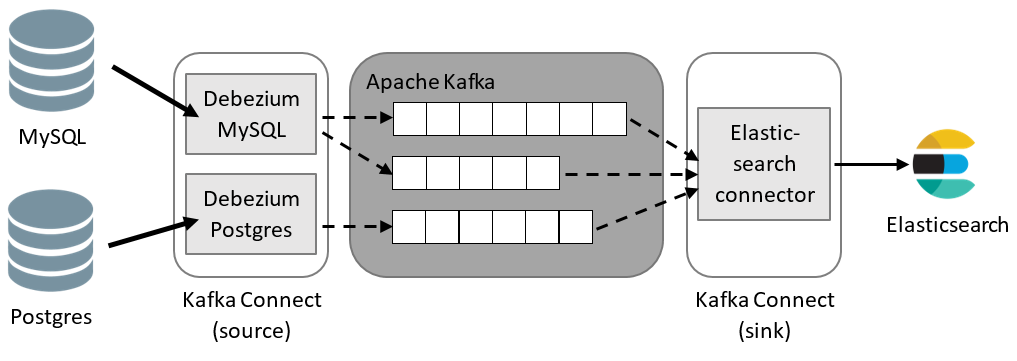
\includegraphics[width=0.8\textwidth]{figures/CDC_topology.PNG}
\end{figure}

\end{frame}

\section{Motivácia}

\begin{frame}{Motivácia}

\begin{itemize}
  \item<1-> Parsovanie DDL dotazov
  \begin{itemize}
    \item<1-> Špecifické typy DDL dotazov pre každé DBMS
    \item<1-> Neexistuje použiteľná knižnica
  \end{itemize}
  \item<2-> Aktuálne riešenie DDL parseru
  \begin{itemize}
    \item<2-> Ručne implementované
    \item<2-> \alert{Nekompletná implementácia}
    \item<2-> \alert{Náročné na správu}
  \end{itemize}
\end{itemize}

\end{frame}

\section{Ciele}

\begin{frame}{Ciele}

\begin{enumerate}
  \item Analýza možností nahradenia existujúceho riešenia
  \item Návrhnúť nové riešenie
  \begin{itemize}
    \item Strojovo generovaný parser
    \item Jenoduchý na spávu
  \end{itemize}
  \item Začlenenie nového parseru do projektu Debezium
  \begin{itemize}
    \item Budúca podpora iných DBMS
  \end{itemize}
  \item Otestovanie parseru pomocou testovacej sady projektu Debezium
\end{enumerate}

\end{frame}

\section{Syntaktická analýza}

\begin{frame}{Syntaktická analýza}

\begin{itemize}
  \item Teoreticky vyriešenný problém
  \begin{itemize}
    \item \textit{Top-Down} parsovanie - LL gramatiky
    \item \textit{Bottom-Up} parsovanie - LR gramatiky
  \end{itemize}
  \item V praxi sa stále vylepšuje  
  \begin{itemize}
    \item 2008 $\rightarrow$ \textbf{Bison} - IELR gramatika
    \item 2014 $\rightarrow$ \textbf{ANTLR v4} - ALL(*) gramatika
  \end{itemize}
\end{itemize}

\begin{figure}
\centering
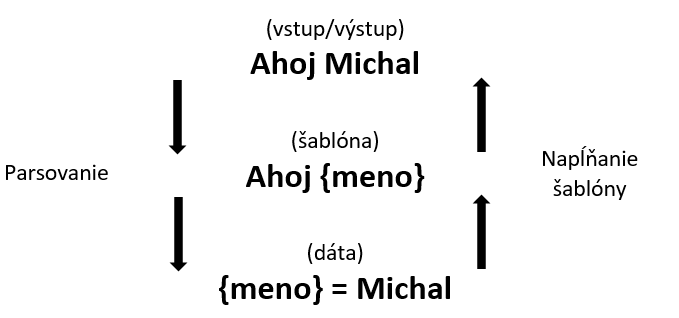
\includegraphics[width=0.5\textwidth]{figures/templatingAndParsing.PNG}
\end{figure}

\end{frame}

\section{ANTLR v4}

\begin{frame}{ANTLR v4}

\begin{itemize}
  \item<1-> Veľká komunita užívateľov
  \item<2-> Mnoho podporných nástrojov
  \item<3-> Odstraňuje priamu ľavú rekurziu
  \item<4-> \alert{Dostupný repozitár vytvorených gramatík}
\end{itemize}

\begin{figure}
\centering
\visible<2->{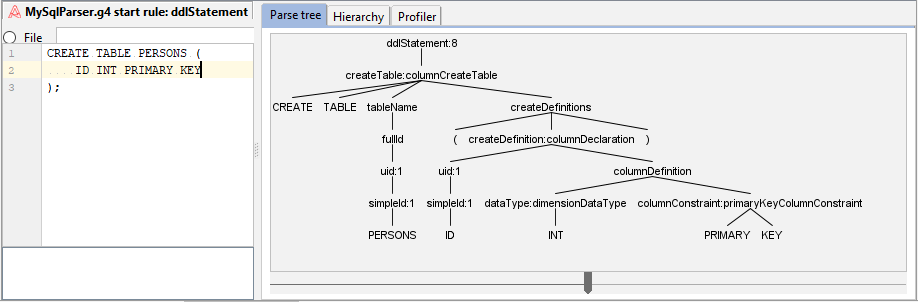
\includegraphics[width=0.8\textwidth]{figures/antlrWorks.PNG}}
\end{figure}

\end{frame}

\section{Dosiahnuté výsledky}

\begin{frame}{Dosiahnuté výsledky}

\begin{itemize}
  \item<1-> Objavenie neregistrovaných chýb existujúceho parseru
  \only<1>{
    \begin{itemize}
      \item Nesprávne chovanie parseru
      \item Podpora syntakticky nevalidných dotazov
    \end{itemize}
  }
  \item<2-> Nový design pre parsovanie DDL
  \only<2>{
    \begin{itemize}
      \item Generalizácia existujúcej implementácie
      \item Generalizácia novej implementácie
      \item Samostatný modul pre generovanie DDL parserov
    \end{itemize}
  }
  \item<3-> Doplnenie chýbajucej implementácie
  \only<3>{
    \begin{itemize}
      \item Parsovanie pohľadových dotazov (\textit{VIEW})
      \item Generalizácia novej implementácie
      \item Samostatný modul pre generovanie DDL parserov
    \end{itemize}
  }
  \item<4-> Oprava nevalidných testov
  \only<4>{
    \begin{itemize}
      \item Syntakticky nesprávne dotazy
      \item Oprava použitej gramatiky
      \item Implementácia nových testov
    \end{itemize}
  }
  \item<5-> Začlenenie parseru do projektu Debezium
  \only<5>{
    \begin{itemize}
      \item Možnosť voľby parsovacej strategie
      \item Akceptovanie \textit{coding rules} projektu
    \end{itemize}
  }
\end{itemize}

\end{frame}

\section{Poďakovanie}
\begin{frame}
\centering\Large Ďakujem za pozornosť
\vspace{2em}

\centering\normalsize
Bc. Roman Kuchár\\ kucharrom@gmail.com
\end{frame}

% \appendix
% \subsection{Otázka oponenta}
% \begin{frame}{Otázka oponenta}
% \begin{block}{Otázka}
% Dosažené v\'ysledky umožňují oddělit služby od byznysov\'ych pravidel, což by v případě rozsáhl\'ych informačních systémů přirozeně vedlo k rozdělení kompetencí, kdy by v\'yvojář měl na starost kód služby a doménov\'y expert by spravoval byznysová pravidla ve formě DSL. Průsečíkem jejich práce by byl název byznysového kontextu, což poskytuje mnoho prostoru pro chybnou interpretaci. V\'yvojář může mylně předpokládat, že byznysov\'y kontext nahrazuje funkcionalitu, která měla b\'yt ve skutečnosti implementována jako součást služby. Obdobná situace platí pro doménového experta. V\'ysledkem mohou b\'yt chyby aplikace, nekonzistence dat nebo bezpečnostní rizika. \alert{Nevytváří řešení jednoho problému novou třídu úplně jin\'ych problémů spojen\'ych s lidsk\'ym faktorem?}
% \end{block}
% \end{frame}

% \begin{frame}{Otázka oponenta}
% \begin{block}{Odpověď}
% \begin{itemize}
% \item<1-> Lidský faktor obecně hraje nezabedbatelnou roli při vývoji informačních systémů
% \item<2-> Při vývoji informačních systému je nutná komunikace mezi vývojáři a doménovými experty, ale i ostatními stakeholdery
% \item<3-> Byznysový kontext by bylo možné doplnit o dokumentační komentář, který by pomohl doménovým expertům a vývojářům lépe komunikovat jednotlivé zodpovědnosti
% \item<4-> Výsledný systém je potřeba důkladně testovat, aby případné chyby byly odhaleny
% \item<5-> Děkuji oponentovi za konstruktivní otázku
% \end{itemize}
% \end{block}
% \end{frame}

\end{document}
